\documentclass[../../main.tex]{subfiles}

\begin{document}
\subsection{Internet Checksum}
\begin{definition}
    Fix a bit sequence of size $M\times l$, we can view this as a matrix with $m$ rows and $l$ columns. If $d$ is the sequence, then
    \[d = \begin{bmatrix}d_1,\, d_2,\,\cdots,\,d_m\end{bmatrix}\]
    Where each $d_m$ is a vector of size $l$ on its own. So $d$ is a vector containing vectors.\\
    
    The checksum $d_0$ is defined inductively. For each $1\leq m\leq M$,
    \begin{itemize}
        \item We first initialize $d_0 = \vec{0}$, and
        \item for each $m\in[1,M]$, $d_0 = d_m + d_0$. This is done by one's complement addition.\\
        
        One's Complement Addition, fix two vectors of size $l$, $\vec{x}$, $\vec{y}$, and consider their binary representations, and add them together.
        \[
        \vec{x} + \vec{y} = \biggl(\sum_{i=0}^{l-1} x_i 2^i\biggr) + \biggl(\sum_{i=0}^{l-1} y_i 2^i\biggr) = \sum_{i=0}^{l} s_i 2^i
        \]
        The result may be a $l+1$ digit number. If this is so, then the carry-out of the sum is added again to the result. Do this for all $m\leq M$.\\
        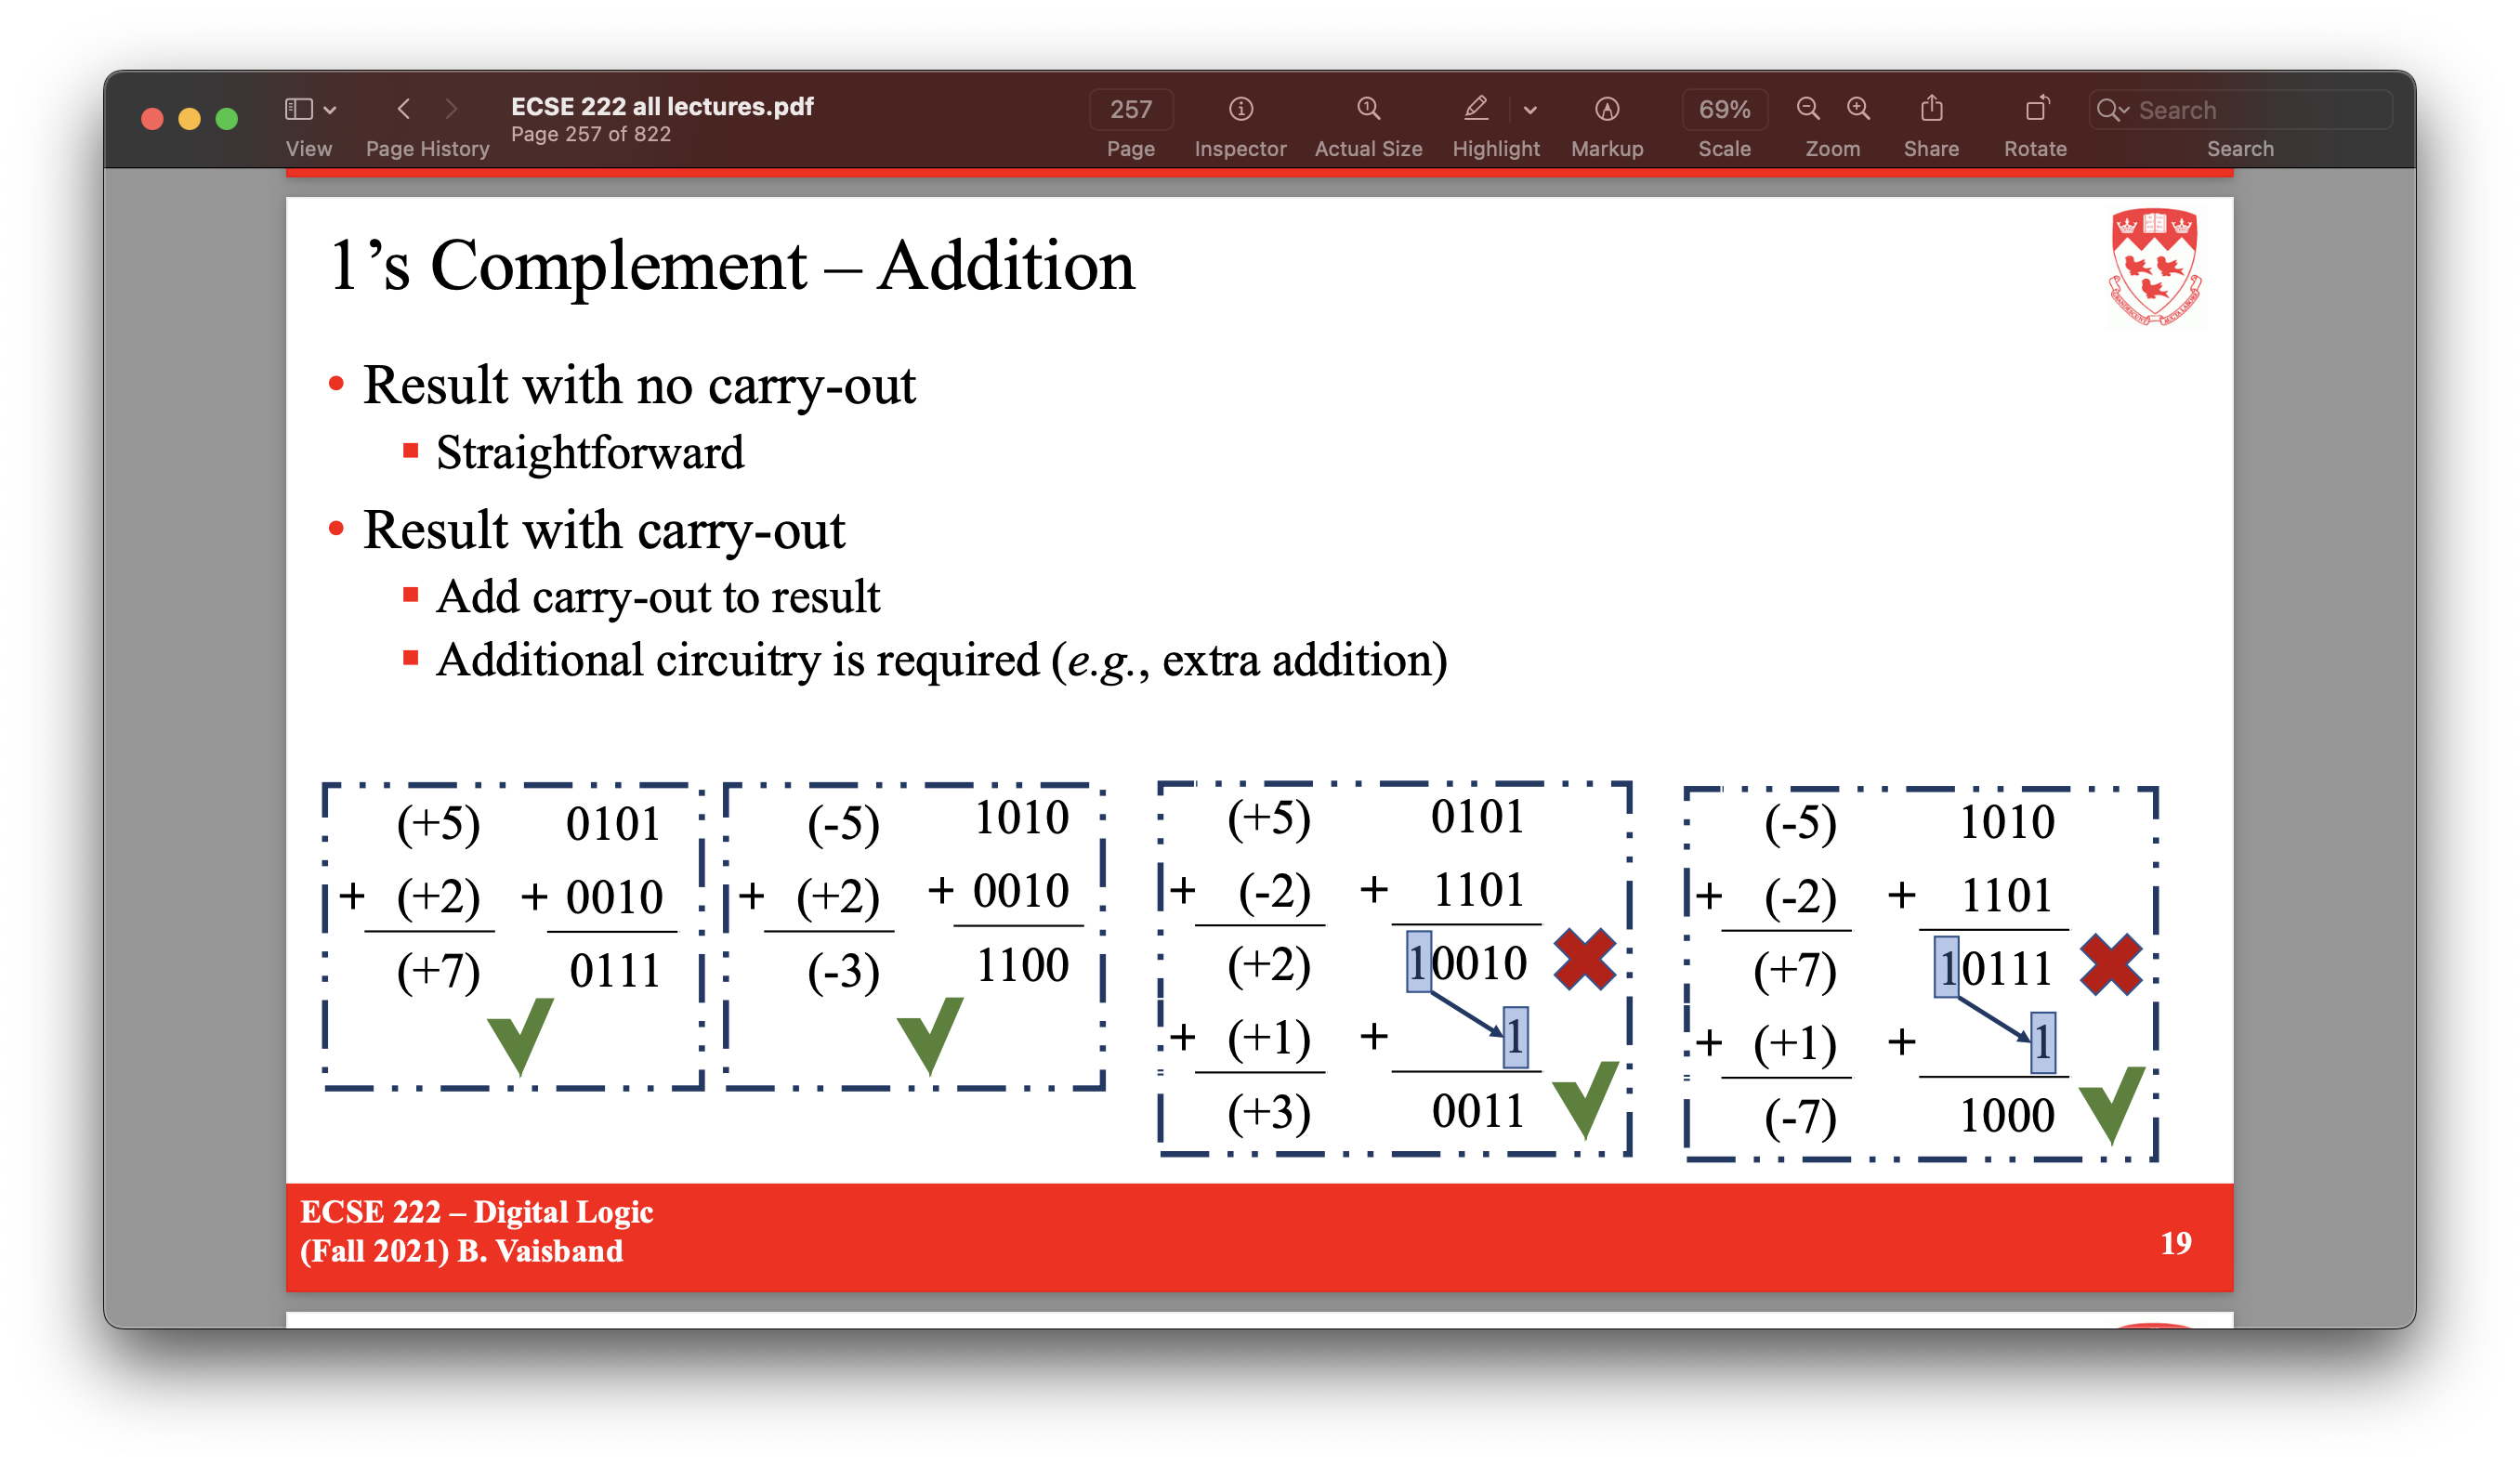
\includegraphics[width=\textwidth]{images/ones_complement_addition.png}
        \item At the end of the process, flip all the bits in $d_0$
        \[
        d_0 = \biggl(1\oplus d_{l-1},\cdots 1\oplus d_{0}\biggr)
        \]
    \end{itemize}
\end{definition}
    The result is the following error-checking scheme.
\begin{wtr}[Internet Checksum]
\begin{enumerate}
        \item[]
        \item If there is no error, then
        \[
        \boxed{\sum_{j\geq 0}^M d_j=0}
        \]
        \item The internet checksum can detect all one-bit error patterns.
        \item For a sequence of bits divided in $M$ chunks, the transmitted sequence has $M+1$ chunks.
        \item The internet checksum $d_0$ is obtained by adding all $d_j$ in one's complement, and flipping all the bits (like in one's complement).
    \end{enumerate}
\end{wtr}    


\end{document}